% Shared standalone design for the editable figure reconstructions.
\documentclass[tikz,border=5pt,10pt]{standalone}
\usepackage[T1]{fontenc}
\usepackage[utf8]{inputenc}
\usepackage{newpxtext,newpxmath}
\usepackage[scaled=.94]{sourcesanspro}
\usepackage{pgfplots}
\pgfplotsset{compat=1.18}
\usetikzlibrary{arrows.meta,calc,positioning,decorations.pathreplacing,
  decorations.markings,patterns,matrix,shapes.geometric,fit,backgrounds,
  intersections,angles,quotes}
\definecolor{ink}{HTML}{203746}
\definecolor{accent}{HTML}{146C78}
\definecolor{muted}{HTML}{667780}
\definecolor{signalred}{HTML}{B94B44}
\color{ink}
\tikzset{>=Latex,line width=.8pt,
  every node/.style={font=\small},
  axis/.style={->,draw=muted,line width=.5pt},
  guide/.style={draw=muted,dashed,line width=.45pt},
  curve/.style={draw=accent,line width=1pt},
  marker/.style={circle,fill=accent,inner sep=1.5pt},
  labelbox/.style={fill=white,inner sep=2pt}}

\begin{document}
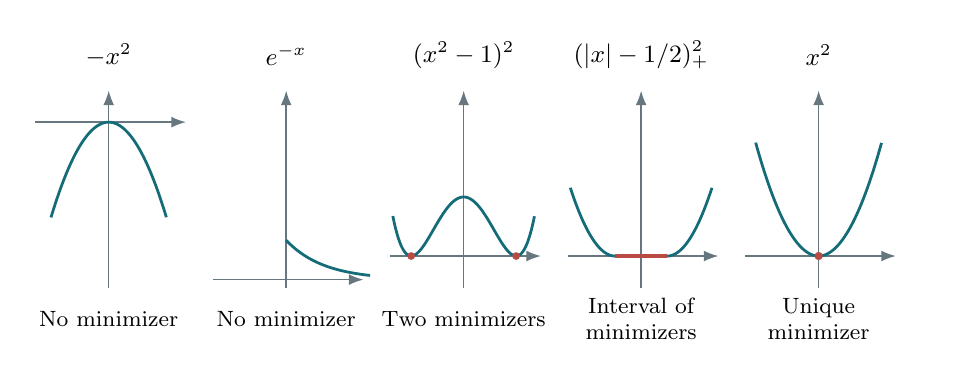
\begin{tikzpicture}[x=.98cm]
\path[use as bounding box] (-.25,-.85) rectangle (11.5,3.2);\begin{scope}[shift={(0.8,0)}]
\draw[axis] (-.95,2)--(1.0,2);\draw[axis] (0,-.1)--(0,2.4);\begin{scope}[xscale=.68]\draw[curve] plot[domain=-1.1:1.1,samples=101] (\x,{2-\x*\x});
\end{scope}\node at (0,2.85) {$-x^2$};\node[align=center,text width=2.1cm,font=\footnotesize] at (0,-.5) {No minimizer};
\end{scope}
\begin{scope}[shift={(3.0999999999999996,0)}]
\draw[axis] (-.95,0)--(1.0,0);\draw[axis] (0,-.1)--(0,2.4);\begin{scope}[xscale=.68]\draw[curve] plot[domain=.0:1.6,samples=101] (\x,{exp(-1.4*\x)*.5});
\end{scope}\node at (0,2.85) {$e^{-x}$};\node[align=center,text width=2.1cm,font=\footnotesize] at (0,-.5) {No minimizer};
\end{scope}
\begin{scope}[shift={(5.3999999999999995,0)}]
\draw[axis] (-.95,.3)--(1.0,.3);\draw[axis] (0,-.1)--(0,2.4);\begin{scope}[xscale=.68]\draw[curve] plot[domain=-1.35:1.35,samples=101] (\x,{.75*(\x*\x-1)^2+.3});
\end{scope}\node at (0,2.85) {$(x^2-1)^2$};\node[align=center,text width=2.1cm,font=\footnotesize] at (0,-.5) {Two minimizers};\fill[signalred] (-.68,.3) circle (1.4pt) (.68,.3) circle (1.4pt);
\end{scope}
\begin{scope}[shift={(7.699999999999999,0)}]
\draw[axis] (-.95,.3)--(1.0,.3);\draw[axis] (0,-.1)--(0,2.4);\begin{scope}[xscale=.68]\draw[curve] plot[domain=-1.35:1.35,samples=101] (\x,{1.2*max(abs(\x)-.5,0)^2+.3});
\end{scope}\node at (0,2.85) {$(|x|-1/2)_+^2$};\node[align=center,text width=2.1cm,font=\footnotesize] at (0,-.5) {Interval of minimizers};\draw[signalred,line width=1.6pt] (-.34,.3)--(.34,.3);
\end{scope}
\begin{scope}[shift={(10.0,0)}]
\draw[axis] (-.95,.3)--(1.0,.3);\draw[axis] (0,-.1)--(0,2.4);\begin{scope}[xscale=.68]\draw[curve] plot[domain=-1.2:1.2,samples=101] (\x,{\x*\x+.3});
\end{scope}\node at (0,2.85) {$x^2$};\node[align=center,text width=2.1cm,font=\footnotesize] at (0,-.5) {Unique minimizer};\fill[signalred] (0,.3) circle (1.5pt);
\end{scope}

\end{tikzpicture}
\end{document}
